\documentclass[tikz,border=1.35mm]{standalone}

\definecolor{fvmadaptedge}{HTML}{8A7E7E}
\usetikzlibrary{arrows.meta}

\definecolor{externalface}{HTML}{8FB9E8}
\definecolor{splitred}{HTML}{AF2525}
\definecolor{centroidgreen}{HTML}{0E8814}

% Centroidal refinement scaffold for a tetrahedron.
% Face centroids connect to edge midpoints in red, and face centroids connect
% to the volume centroid in green.
\begin{document}
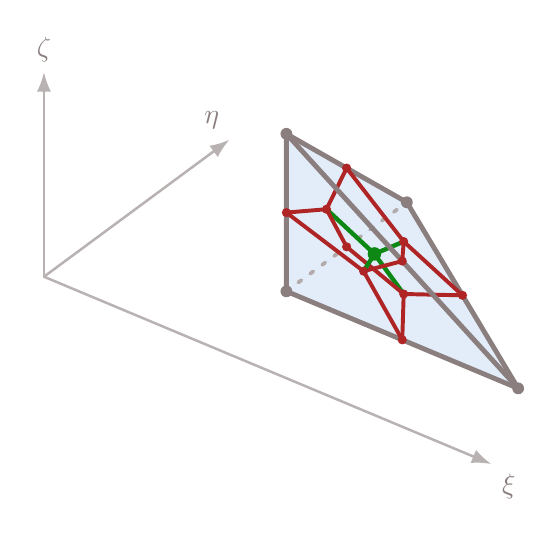
\begin{tikzpicture}[
  x={(20.3mm,-8.5mm)},
  y={(15.3mm,11.3mm)},
  z={(0mm,20mm)},
  line join=round,
  line cap=round,
  outer/.style={draw=fvmadaptedge,line width=0.62mm},
  hidden/.style={draw=fvmadaptedge!65,line width=0.48mm,loosely dotted},
  face/.style={fill=externalface,fill opacity=0.14,draw=none},
  split/.style={draw=splitred,line width=0.50mm},
  centroidedge/.style={draw=centroidgreen,line width=0.56mm},
  axis/.style={draw=fvmadaptedge!60,line width=0.32mm,-{Latex[length=2.5mm,width=1.8mm]}}
]
  % Reference tetrahedron vertices.
  \coordinate (A) at (0,0,0);
  \coordinate (B) at (1.45,0,0);
  \coordinate (C) at (0,1,0);
  \coordinate (D) at (0,0,1);

  % Edge midpoints.
  \coordinate (mAB) at (0.725,0,0);
  \coordinate (mAC) at (0,0.5,0);
  \coordinate (mAD) at (0,0,0.5);
  \coordinate (mBC) at (0.725,0.5,0);
  \coordinate (mBD) at (0.725,0,0.5);
  \coordinate (mCD) at (0,0.5,0.5);

  % Face centroids and volume centroid.
  \coordinate (fABC) at (0.483,0.333,0);
  \coordinate (fABD) at (0.483,0,0.333);
  \coordinate (fACD) at (0,0.333,0.333);
  \coordinate (fBCD) at (0.483,0.333,0.333);
  \coordinate (center) at (0.3625,0.25,0.25);

  % Offset computational-coordinate axes.
  \coordinate (Oaxis) at (-1.20,-0.42,-0.18);
  \draw[axis] (Oaxis) -- (1.60,-0.42,-0.18) node[below right,font=\normalsize,text=fvmadaptedge] {$\xi$};
  \draw[axis] (Oaxis) -- (-1.20,1.12,-0.18) node[above left,font=\normalsize,text=fvmadaptedge] {$\eta$};
  \draw[axis] (Oaxis) -- (-1.20,-0.42,1.12) node[above,font=\normalsize,text=fvmadaptedge] {$\zeta$};

  % Exterior faces remain faint so the refinement scaffold is legible.
  \path[face] (A) -- (B) -- (C) -- cycle;
  \path[face] (A) -- (B) -- (D) -- cycle;
  \path[face] (A) -- (C) -- (D) -- cycle;
  \path[face] (B) -- (C) -- (D) -- cycle;

  % Hidden geometry is drawn before the refinement construction.
  \draw[hidden] (A) -- (C);

  % Green face-centroid to volume-centroid connections.
  % The x-z face link is drawn later so it appears in front of the crossing
  % red split on the bottom x-y face.
  \foreach \p in {fABC,fACD,fBCD} {
    \draw[centroidedge] (center) -- (\p);
  }

  % These face splits pass behind the visible x-z edge from D to B.
  \draw[split] (fABC) -- (mBC);
  \draw[split] (fACD) -- (mCD);

  % Visible exterior wireframe occludes internal centroid connections.
  \draw[outer] (A) -- (B);
  \draw[outer] (A) -- (D) -- (B);
  \draw[outer] (B) -- (C) -- (D);

  % Red face-centroid splits on all four original faces.
  \foreach \p in {mAB,mAC} {
    \draw[split] (fABC) -- (\p);
  }
  \foreach \p in {mAB,mBD,mAD} {
    \draw[split] (fABD) -- (\p);
  }
  \foreach \p in {mAC,mAD} {
    \draw[split] (fACD) -- (\p);
  }
  \foreach \p in {mBC,mCD,mBD} {
    \draw[split] (fBCD) -- (\p);
  }

  % Draw this centroid connection after the red splits to match the view depth.
  \draw[centroidedge] (center) -- (fABD);

  % Visible original vertices are #8a7e7e.
  \foreach \p in {A,B,C,D} {
    \fill[fvmadaptedge] (\p) circle[radius=0.75mm];
  }

  % Face and edge refinement nodes are red.
  \foreach \p in {mAB,mAC,mAD,mBC,mBD,mCD,fABC,fABD,fACD,fBCD} {
    \fill[splitred] (\p) circle[radius=0.58mm];
  }
  \fill[centroidgreen] (center) circle[radius=0.86mm];
\end{tikzpicture}
\end{document}
